\documentclass[main.tex]{subfiles} % Subfile-Class


% ============================================================================== %
%                            Subfile document                                    %
% ============================================================================== %

\begin{document}

% Template

\subsubsection{Chassis und Fahrwerk}

Dieser Abschnitt behandelt die Evaluierung des Fahrwerks in Bezug auf die
Radauswahl und die Chassis-Konstruktion. Dabei werden verschiedene
Konzeptlösungen diskutiert und getestet. Abschliessend wird die finale
Entscheidung auf Basis der Testergebnisse dokumentiert.

% ===================================================================================
\subsubsection*{Anforderungen}

\textbf{Gewicht:} \newline
Das Gewicht stellt, wie auch bei allen anderen Baugruppen, einen kritischen Faktor dar.
Daher basiert das Chassis auf dem Konzept einer einzigen Grundplatte, anstatt einen
Volumenkörper zu entwerfen, der sämtliche Aktoren, Sensoren und Steuerungskomponenten
umschliesst. Wie eine Abdeckung für das Gerät aussehen wird, steht noch offen. 
Zudem wird angestrebt, die Konstruktion auf zwei Räder zu beschränken.
Die Drehbewegung wird mittels Skid Steering realisiert. Um die Stabilität zu
gewährleisten, benötigt der Roboter jedoch einen dritten Auflagepunkt, dessen genaue
Umsetzung im Nachfolgemodul PREN 2 durch verschiedene Tests untersucht wird.

\textbf{Geschwindigkeit:} \newline
Da die Motoren bereits ausgewählt sind und ihre Drehzahl technisch begrenzt ist,
kann die maximale Fahrgeschwindigkeit lediglich über die Radgrösse definiert werden.
Von einem Getriebe wird bewusst abgesehen, um Gewicht und Kosten zu reduzieren.

\textbf{Kosten:} \newline
Die Anbauteile des Chassis werden mit einem 3D-Drucker gefertigt, da dem Team
25 Stunden Druckzeit des HSLU-T\&A-Druckers kostenfrei zur Verfügung stehen.
Die Kosten für die Räder sollen unter 20 CHF bleiben, um ein grösseres Budget
für kritische Funktionen bereitzustellen.

% ===================================================================================
\subsubsection*{Konzeptionierung}

Die Grundplatte des Chassis wird aus einer MDF-Platte gefertigt, in die
sämtliche Ausschnitte und Öffnungen mittels Lasergravur eingebracht werden.
Komponenten werden modular mit Anbauteilen aus dem 3D-Druck auf der Grundplatte
montiert. Diese modulare Konstruktion ermöglicht einfache Anpassungen und
hilft, das Gewicht zu reduzieren.

Bereits früh in der Projektphase wurde entschieden, dass die Fortbewegung des
Pfadfinders mit zwei Rädern und einem dritten Auflagepunkt realisiert werden
soll. Abbildung~\ref{fig:Radkonzept} zeigt eine erste Konzeptskizze des
Chassis, einschliesslich der Räder und einer Rutschfläche als drittem
Auflagepunkt.

\begin{figure}[H]
    \centering
    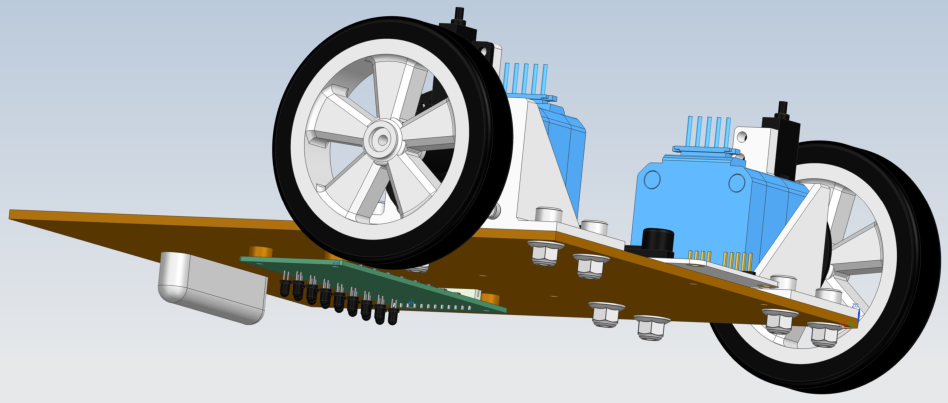
\includegraphics[width=0.75\textwidth]{Radkonzept.pdf}
    \caption{Chassis Konzept in Siemens NX}~\label{fig:Radkonzept}
\end{figure}

Die Räder dürfen eine maximale Breite von 20 mm nicht überschreiten, um
ausreichend Platz auf der Grundplatte für Motoren und Motorentreiber
bereitzustellen. Der Mindestdurchmesser beträgt 80 mm, da andernfalls die
Liniensensoren nicht wie vorgesehen montiert werden können. Zudem ermöglicht
ein grösserer Durchmesser von 80 mm eine maximale Geschwindigkeit von
1.676~m/s, was den Projektanforderungen entspricht. Die Berechnung erfolgt
gemäss folgender Formel:

\[ v_{max} = n_{Motor} \cdot d_{Rad} \cdot \pi = 1.676 \, \frac{\text{m}}{\text{s}} \]

Auf Grundlage der genannten Anforderungen wurde auf verschiedenen Webseiten
nach passenden Rädern gesucht. Die Ergebnisse sind in
Tabelle~\ref{tab:Rad_Parameter} zusammengefasst.

\begin{table}[h]                                    % h = here
    \centering
    \begin{tabular}{|c|c|c|c|c|c|}                        % c=centered, l=left, r=right
        \hline
        Hersteller & Herst. Nr. & Preis    & Durchmesser & Material   & Gewicht \\
                   &            &          &             & Lauffläche &         \\ \hline
        ServoCity  & 595660     & 9.05 CHF & 80.3 mm     & Silikon    & 19 g    \\ \hline
        DF-Robot   & FIT0500    & 2.62 CHF & 80 mm       & Silikon    & -       \\ \hline
    \end{tabular}
    \caption{Rad Parameter}
    \label{tab:Rad_Parameter}
\end{table}

% ===================================================================================
\subsubsection*{Entscheidung und Fazit}
Von den beiden untersuchten Rädern wurde das Modell FIT0500 von DF-Robot ausgewählt.
Obwohl die Aufnahme des ServoCity-Rades technisch besser geeignet wäre, wurden die
erheblichen Lieferkosten von 70 CHF als entscheidender Nachteil gewertet.

\end{document}
